\begin{abstract}
Forecasting requires structure: deciding which evidence bears on an outcome,
which relationship applies, and when observations should revise it. We ask
whether language models (LMs) forecast by selecting, revising, and transferring
such relationships across real markets and controlled tasks\footnote{%
  \micon{huggingface.png}\;%
  \href{https://huggingface.co/datasets/anonymous-review/forecasting-study-data}%
  {Study dataset and artifacts}\quad
  \micon{gh_logo.png}\;%
  \href{https://github.com/anonymous-review/forecasting-study-code}%
  {Code repository}. Links anonymized for review.%
}.
Across these settings, models update selectively, use context to choose among
competing predictive relationships, revise those choices as evidence accumulates,
and infer mappings whose meanings change across episodes. Internal representations
track these behavioral distinctions, and a targeted intervention can alter a
forecast. Training aligned with episode structure improves transfer, while
proper-score training improves forecasts on sealed markets. These effects vary
across model families and scale and do not establish superiority to forecasting
crowds. Together, the results support a view of LM forecasting as
context-dependent structural induction.
\end{abstract}
\section{Introduction}
\label{sec:introduction}
\begin{wrapfigure}{r}{0.52\textwidth}
\vspace{-2.0em}
\centering
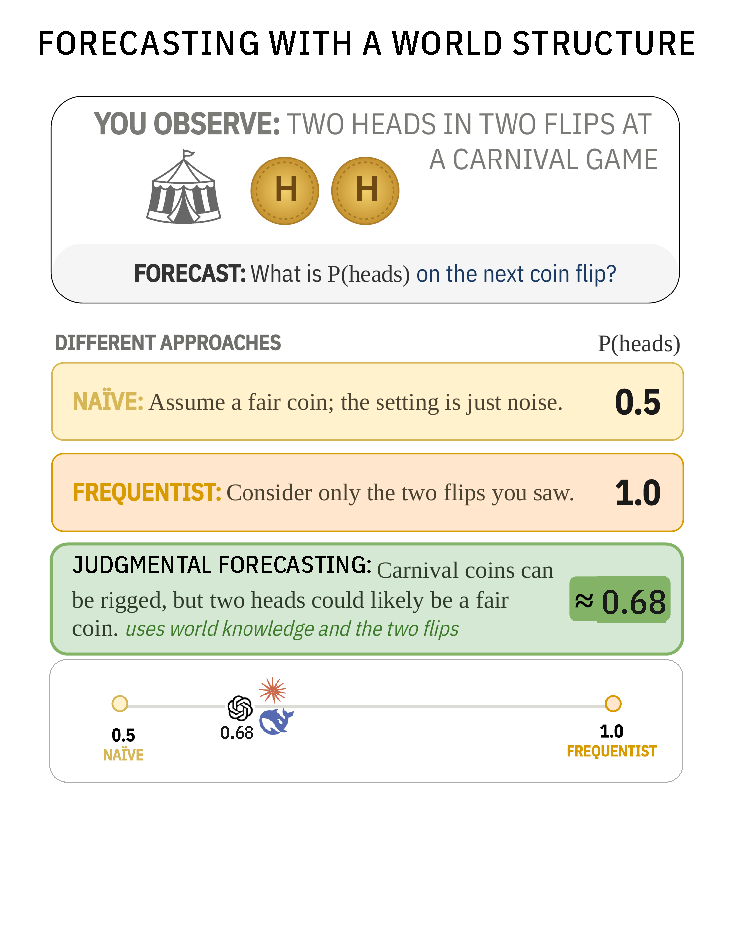
\includegraphics[width=\linewidth,trim=0 72pt 0 0,clip]{figures/teaser_revised.pdf}
\vspace{-0.6cm}
\caption{ \textbf{A descriptive probe motivates relationship selection.}
\small
After two heads from an unfamiliar carnival coin, mean next-head forecasts are
$.644$, $.681$, and $.712$ for GPT-5.4, Claude Opus~4.8, and DeepSeek V4-Pro,
respectively, over 8 temperature-$0.7$ calls each. This single condition
illustrates, but does not identify, the relationship being applied
(Appendix~\ref{app:carnival-coin-probe}).}
\vspace{-0.5cm}
\label{fig:world-knowledge-evidence}
\end{wrapfigure}

Language models (LMs) approach crowd forecasting accuracy, and ensembles
match it on some question sets \citep{halawi2024approaching,schoenegger2024wisdom}.
Results on Metaculus, Polymarket, and Kalshi
\citep{lu2025evaluating,cao2026auditable,zhang2026prediction} therefore raise a
process question: \emph{why are LMs competitive forecasters?} The same probability
can come from a base rate, a retrieved case, a market signal, or a predictive
relationship. Pointwise accuracy cannot distinguish these strategies, especially
when they agree on familiar questions but diverge after a change in context.

Figure~\ref{fig:world-knowledge-evidence} illustrates the distinction. For a
known-fair coin, the first two flips do not change the next-flip probability from
$0.5$; for a coin of unknown bias, the same observations can be informative.
Asked about an unfamiliar carnival coin, three systems answer near $0.68$, away
from the fixed fair-coin reference. The probe has only one condition and motivates
rather than identifies the relationship being applied
(Appendix~\ref{app:carnival-coin-probe}). The question it exposes is central to
\textbf{judgmental forecasting}, which combines base rates, sparse observations,
qualitative evidence, and domain knowledge to estimate future events
\citep{mellers2014psychological,tetlock2016superforecasting}.


We ask whether LM forecasts exhibit behavioral signatures of this process, which
we call \emph{inductive reasoning}: selecting a predictive relationship from
context and sparse observations, revising that selection as evidence accumulates,
and applying the relationship to a new case
\citep{tenenbaum2006theory,griffiths2010probabilistic,lake2017building}.
We use \emph{world structure} for the predictive relationships among variables.
These are behavioral definitions; they presume neither an explicit graph nor a
particular internal representation.

Generated explanations need not reveal this process
\citep{jacovi2020towards,turpin2023language}. We therefore use paired interventions
with predicted changes or invariances \citep{ribeiro2020beyond,elazar2021measuring}:
vary evidence direction within a topic, reverse a context--regime assignment while
holding numerical inputs fixed, add observations that conflict with a cue, and
preserve the distribution of training answers while breaking their episode-level
correspondence.

\subsection{Empirical Progression}
\label{sec:forecasting-as-inductive}

The four experiments form a progression organized by three questions:
\begin{itemize}[nosep,leftmargin=*]
  \item \textbf{Do LMs react selectively to evidence?
  (\hyperref[sec:exp1]{Experiment~1}).}
  Across 30,094 updates on unresolved real questions, nine models follow the
  withheld packet direction at $.89$--$.99$, versus $.69$ for a market-held-out
  lexical classifier. Seven reviewers reach $.76$ on a smaller categorical
  materials task, not a matched model comparison. Because packet polarity is not
  shown, recovery requires relating the snippet to the market outcome; wording
  nevertheless carries partial signal. Selectivity has two components:
  models return
  the prior unchanged on $1.1$--$71.4\%$ of topically matched controls against
  $0.0$--$1.4\%$ of directional packets, and move $1.9$--$7.5\times$ farther on
  directional packets when they move at all. Their product is the unconditional
  $1.9$--$24.2\times$ ratio. The arms differ in wording, and the relationships
  involved are ones models already hold.
  \item \textbf{Can an LM select a relationship based on context?
  (\hyperref[sec:exp2]{Experiment~2}).}
  A cue selects one of two displayed response regimes: reversing it reverses
  forecasts, and target observations weaken its effect. When arbitrary cue meanings
  change across episodes, twelve of fifteen systems recover the episode-specific
  mapping, including all hosted systems tested. On sealed episodes, linear probes
  across seven open checkpoints decode the induced mapping exactly where forecasts
  recover it, and patching Qwen3-14B's representation moves its zero-shot forecast.
  \item \textbf{Are finetuned LMs able to transfer contextual relationships?
  (\hyperref[sec:exp3]{Experiments~3} and~\hyperref[sec:exp4]{4}).}
  Under joint domain-and-mechanism shift, Qwen3-8B episode-matched response MAE is
  $.25$ $[.06,.47]$ lower than the population-prior control, with the same direction
  at 4B. On a separate 318-market holdout, proper-score training improves every
  mean Brier relative to every tested Qwen and Llama base checkpoint, but the
  trained Qwen series is nonmonotonic
  across 1.7B--14B. The 14B score differs from the contemporaneous Polymarket crowd
  by $+.0004$ $[-.0003,+.0014]$.
\end{itemize}
